\documentclass[b4paper, landscape, dvipdfmx]{jsarticle}
%----- 必要なパッケージ -----
\usepackage{fancybox,ascmac,otf,ulem}
\usepackage{amssymb, amsthm}
\usepackage[leqno]{amsmath}
\usepackage{wrapfig}
\usepackage{geometry}
\usepackage{multicol}
\usepackage{tcolorbox}
\usepackage{xcolor}
\usepackage{fancyhdr}
\usepackage{tikz}

% shadowsライブラリ
\usetikzlibrary{
    positioning,
    arrows.meta,
    calc,
    shadows,
    shadows.blur,
    intersections
}

\tcbuselibrary{skins, breakable, theorems}
\usepackage{enumitem}
\setlist[enumerate,1]{label=(\arabic*)}
\setlist[itemize]{leftmargin=*}
\newcommand{\ds}{\displaystyle}

%----- レイアウト設定 -----
\geometry{
  left=15mm,
  right=15mm,
  top=20mm,
  bottom=15mm,
  headheight=25pt
}

%----- 数式環境の上下の余白調整 -----
\AtBeginDocument{
  \setlength{\abovedisplayskip}{5pt}
  \setlength{\belowdisplayskip}{5pt}
  \setlength{\abovedisplayshortskip}{0pt}
  \setlength{\belowdisplayshortskip}{3pt}
}

%===========================================================
%  デザイン設定(白黒印刷対応・ハイコントラスト)
%===========================================================

%--- 色の定義 ---
% 印刷時にしっかり濃く出るように調整
\definecolor{printBlue}{RGB}{0, 50, 100}     % 濃紺(例題・解説)
\definecolor{printRed}{RGB}{140, 20, 20}     % 濃エンジ(練習・重要)
\definecolor{printTeal}{RGB}{0, 60, 60}      % 濃い青緑(全体課題)
\definecolor{gridColor}{gray}{0.75}          % 解答欄の方眼(印刷飛び防止のため少し濃く)

%===========================================================
%  カラー定義 (calculus_01.tex より復元)
%===========================================================
\definecolor{chartBlue}{RGB}{0, 65, 120}   % 青チャート風ネイビー
\definecolor{chartRed}{RGB}{160, 20, 20}   % 重要用エンジ色
\definecolor{chartTeal}{RGB}{0, 100, 100}  % 全体課題用(青緑)
\definecolor{chartOrange}{RGB}{200, 100, 0}% まとめ用

%===========================================================
%  TikZスタイル定義 (calculus_01.tex より復元)
%===========================================================
\tikzset{
    % 共通のブロックスタイル
    block/.style={
        rectangle,
        rounded corners=4pt,     % 角の丸み
        draw=black!60,           % 枠線の色
        thick,
        fill=white,
        text width=8.5cm,        % 幅(2段組用に調整、1カラムなら12cm等へ変更可)
        align=left,              % 左寄せ
        inner sep=3mm,           % 内側の余白
        font=\sffamily,          % フォント
        % 影の設定
        drop shadow={opacity=0.2, shadow xshift=2pt, shadow yshift=-2pt} 
    },
    % 矢印のスタイル
    arrow/.style={
        ->,
        % 矢印の先端を「Stealth(ステルス機型)」
        >={Stealth[round, length=3mm, width=2mm]}, 
        color=black!60,          % 色
        line width=1.5pt,        % 太さ
        shorten <= 3pt,          % 始点の余白
        shorten >= 3pt           % 終点の余白
    }
}

%--- 共通スタイル定義 ---
\tcbset{
    chartbox/.style={
        enhanced,
        fonttitle=\sffamily\bfseries,
        boxrule=1pt,
        arc=2pt,
        top=1.0em,
        nobeforeafter,
        enlarge left by=-2mm,
        enlarge right by=-2mm,
        drop fuzzy shadow,
        colback=white, % 背景を白に固定(コピー対策)
        attach boxed title to top left={xshift=10pt, yshift*=-\tcboxedtitleheight/2},
        boxed title style={frame hidden, sharp corners, rounded corners=southeast, arc=3pt}
    }
}

% 1. 「全体課題」用のボックス環境
\newenvironment{overall}[1]{
\begin{tcolorbox}[
    chartbox,
    colframe=printTeal,
    coltitle=white,
    title=\textbf{全体課題 #1},
    boxed title style={colback=printTeal},
]}
{\end{tcolorbox}}

% 5. 解説・雑記用(any環境:黒枠・白背景)
\newenvironment{any}[1]{
    \begin{tcolorbox}[
        enhanced,
        colframe=black,       % 真っ黒に変更してくっきりさせる
        colback=white,
        coltitle=white,
        title=\textbf{#1},
        fonttitle=\sffamily,
        attach boxed title to top left={xshift=3mm, yshift*=-\tcboxedtitleheight/2},
        boxed title style={frame hidden, colback=black, sharp corners, rounded corners=northeast, arc=3pt},
        boxrule=1pt,
        arc=2pt,
        top=1em,
        nobeforeafter,
        enlarge left by=-2mm,
        enlarge right by=-2mm,
        segmentation style={draw=black!60, dashed}
    ]}
{ \end{tcolorbox}}

% 6. 例題用(濃紺枠・白背景)
\newenvironment{eg}[1]{
\begin{tcolorbox}[
    chartbox,
    colframe=printBlue,
    coltitle=white,
    title=\textbf{例題 #1},
    boxed title style={colback=printBlue},
    segmentation style={draw=printBlue, line width=0.5pt, dashed}
]}
{\end{tcolorbox}}

% 7. 練習用(濃エンジ枠・白背景)
\newenvironment{prac}[1]{
\begin{tcolorbox}[
    chartbox,
    colframe=printRed,
    coltitle=white,
    title=\textbf{練習 #1},
    boxed title style={colback=printRed}
]}
{\end{tcolorbox}}

\newenvironment{answer}[1][height fill]{
    \begin{tcolorbox}[
        enhanced,
        title={Memo / Answer},
        colframe=black!80,
        colback=white,
        coltitle=black!60,
        fonttitle=\sffamily\bfseries,
        attach boxed title to top left={xshift=5mm, yshift*=-\tcboxedtitleheight/2},
        boxed title style={frame hidden, colback=white},
        boxrule=1pt,
        arc=1pt,
        nobeforeafter,
        enlarge left by=2mm, 
        enlarge right by=2mm, 
        height fill,
        segmentation style={draw=black!20, solid},
        underlay={% 方眼を描画
            \begin{tcbclipinterior}
                \draw[step=5mm, black!5, ultra thin] (interior.south west) grid (interior.north east);
            \end{tcbclipinterior}
        }, 
        #1
    ]}
{ \end{tcolorbox}}

\newenvironment{proofbox}[1][height fill]{
    \begin{tcolorbox}[
        enhanced,
        title={Proof},
        colframe=black!80,
        colback=white,
        coltitle=black!60,
        fonttitle=\sffamily\bfseries,
        attach boxed title to top left={xshift=5mm, yshift*=-\tcboxedtitleheight/2},
        boxed title style={frame hidden, colback=white},
        boxrule=1pt,
        arc=1pt,
        nobeforeafter,
        width=\linewidth,
        underlay={% 方眼を描画
            \begin{tcbclipinterior}
                \draw[step=5mm, black!5, ultra thin] (interior.south west) grid (interior.north east);
            \end{tcbclipinterior}
        },
        #1
    ]}
{ \end{tcolorbox}}

%----- 段組の設定 -----
\setlength{\columnsep}{15mm}
\setlength{\columnseprule}{0.4pt}
\renewcommand{\columnseprulecolor}{\color{black!30}}

%----- ヘッダーの設定 -----
\pagestyle{fancy}
\fancyhf{}

% ヘッダーデザイン
\fancyhead[C]{%
    \begin{tikzpicture}[remember picture, overlay]
        % ヘッダーの帯も濃紺に
        \node[anchor=north west, fill=printBlue, minimum width=\paperwidth, minimum height=5pt] at (current page.north west) {};
    \end{tikzpicture}
}
\fancyhead[L]{\small \textcolor{black!90}{数学\ajRoman{2} $>$ 第1,2章 式と証明/複素数と方程式 $>$ 第1回--\textbf{二項定理}}}
\fancyhead[R]{\small 年 \hspace{1cm} 組 \hspace{1cm} 番 \quad 氏名 \hspace{6cm}}
\renewcommand{\headrulewidth}{0pt}

\begin{document}

\begin{multicols*}{2}

%===========================================================
% 左カラム: 導入・定義・定理
%===========================================================

{\large\textbf{$\clubsuit$学びの全体像}}

\begin{center}
\begin{tikzpicture}[node distance=1.2cm]

    % [1] 整式の計算 (Teal: 基礎)
    \node[block, fill=chartTeal!10, draw=chartTeal] (n1) {
        {\centering \textbf{【第1,2回】 整式の計算と恒等式} \par}
        \vspace{2pt}
        \textbf{\textcolor{chartRed}{「等しい」とはどういうことか}}
        \par \vspace{3pt} \small
        $\bullet$ 二項定理とその仕組み\\
        $\bullet$ 割り算の原理 $A=BQ+R$ の理解\\
        $\bullet$ 恒等式における「係数比較」と「数値代入」の論理
    };

    % [2] 複素数 (Blue: 拡張)
    % n1の下に配置
    \node[block, fill=chartBlue!10, draw=chartBlue, below=of n1] (n2) {
        {\centering \textbf{【第3 $\sim$ 5回】 複素数と方程式} \par}
        \vspace{2pt}
        \textbf{\textcolor{chartRed}{New Game! 数概念の拡張}}
        \par \vspace{3pt} \small
        $\bullet$ 2乗して$-1$になる数 $i$ の導入と計算ルール\\
        $\bullet$ 「解なし」だった2次方程式が解けるようになる世界\\
        $\bullet$ \textbf{注意:}この世界には大小関係が存在しない\\
        $\bullet$解と係数の関係とその成り立ち
    };

    % 分岐させるための座標計算
    % n2の下、左寄りに配置するノードのための座標
    \coordinate[below left=1.5cm and 0.2cm of n2.south] (c_left);
    % n2の下、右寄りに配置するノードのための座標
    \coordinate[below right=1.5cm and 0.2cm of n2.south] (c_right);

    % [3] グラフ (Orange: 視覚化)
    % n2の下に配置(矢印がつながる先)
    \node[block, fill=chartOrange!10, draw=chartOrange, below=of n2] (n3) {
        {\centering \textbf{【第6 $\sim$ 10回】 因数定理とグラフ} \par}
        \vspace{2pt}
        \textbf{\textcolor{chartRed}{式と図形(グラフ)をつなぐ}}
        \par \vspace{3pt} \small
        $\bullet$ 因数定理 $P(\alpha)=0$ による高次方程式の解法\\
        $\bullet$ 方程式の実数解を「グラフと$x$軸の共有点」として視覚化する\\
        $\bullet$ 次章「図形と方程式」への架け橋\\
        $\bullet$到達度テスト
    };

    % [4] 証明 (Red: 実数の本質)
    % n3の下に配置
    \node[block, fill=chartRed!10, draw=chartRed, below=of n3] (n4) {
        {\centering \textbf{【第11 $\sim$ 16回】 式と証明} \par}
        \vspace{2pt}
        \textbf{\textcolor{chartRed}{Real World! 実数の再発見}}
        \par \vspace{3pt} \small
        $\bullet$ 複素数を知った今だからこそわかる\textbf{「実数の強み」}\\
        $\bullet$ $A>B \iff A-B>0$ (大小関係がある)\\
        $\bullet$ $A^2 \geqq 0$ (2乗すると必ず正)\\
        $\bullet$ これらの「実数特権」を駆使して不等式を証明する\\
        $\bullet$単元の総復習
    };

    % 矢印の描画
    \draw[arrow] (n1) -- (n2);
    \draw[arrow] (n2) -- (n3);
    \draw[arrow] (n3) -- (n4);

    % 対比関係を示す破線矢印(複素数 vs 証明)
    % n2(複素数)の右側から出て、大きく迂回してn4(証明)の右側へ
    \draw[<->, dashed, thick, color=black!40] 
        (n2.east) ++(0, 0) -- ++(0.5, 0) 
        |- node[pos=0.25, right, font=\footnotesize, align=left] {対比\\(大小関係の有無)} 
        (n4.east);

\end{tikzpicture}
\end{center}

\columnbreak

{\large \textbf{1. 二項定理の仕組み}}

\begin{any}{パスカルの三角形と係数の法則}
\small
$(a+b)^n$ の展開式について, 係数の並びにどのような規則があるか観察してみよう.

\begin{itemize}
\item $n=0$:
$(a+b)^0=1$
    \item $n=1$: $(a+b)^1 = \mathbf{1}a + \mathbf{1}b$
    \item $n=2$: $(a+b)^2 = \mathbf{1}a^2 + \mathbf{2}ab + \mathbf{1}b^2$
    \item $n=3$: $(a+b)^3 = \mathbf{1}a^3 + \mathbf{3}a^2b + \mathbf{3}ab^2 + \mathbf{1}b^3$
\end{itemize}

これらの係数だけを取り出して並べると, 次のような三角形ができる. これを\textbf{パスカルの三角形}という.

\vspace{1em}
\begin{center}
% ここが修正箇所です。draw=色名 の形に変更しました。
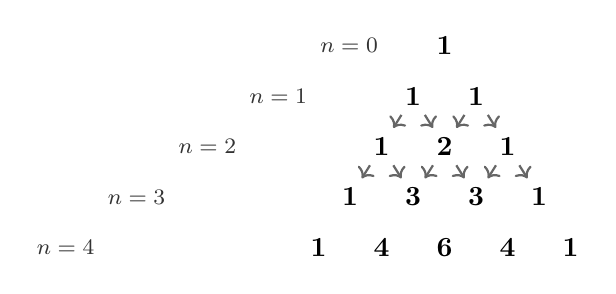
\begin{tikzpicture}[scale=0.8, every node/.style={font=\bfseries}]
    % Rows
    \node (r0) at (0,0) {1};
    \node (r1a) at (-0.5,-0.8) {1}; \node (r1b) at (0.5,-0.8) {1};
    \node (r2a) at (-1,-1.6) {1}; \node (r2b) at (0,-1.6) {2}; \node (r2c) at (1,-1.6) {1};
    \node (r3a) at (-1.5,-2.4) {1}; \node (r3b) at (-0.5,-2.4) {3}; \node (r3c) at (0.5,-2.4) {3}; \node (r3d) at (1.5,-2.4) {1};
    \node (r4a) at (-2,-3.2) {1}; \node (r4b) at (-1,-3.2) {4}; \node (r4c) at (0,-3.2) {6}; \node (r4d) at (1,-3.2) {4}; \node (r4e) at (2,-3.2) {1};
    
    % Arrows (Calculation logic) - 白黒印刷対応のため、半透明(opacity)をやめ、濃いグレーの実線に変更
    \draw[->, draw=black!60, thick] (r1a) -- (r2a);
    \draw[->, draw=black!60, thick] (r1a) -- (r2b); \draw[->, draw=black!60, thick] (r1b) -- (r2b);
    \draw[->, draw=black!60, thick] (r1b) -- (r2c);
    
    \draw[->, draw=black!60, thick] (r2a) -- (r3a);
    \draw[->, draw=black!60, thick] (r2a) -- (r3b); \draw[->, draw=black!60, thick] (r2b) -- (r3b);
    \draw[->, draw=black!60, thick] (r2b) -- (r3c); \draw[->, draw=black!60, thick] (r2c) -- (r3c);
    \draw[->, draw=black!60, thick] (r2c) -- (r3d);
    
    % Labels
    \node[left=0.5cm of r0, font=\footnotesize, black!80] {$n=0$};
    \node[left=1.0cm of r1a, font=\footnotesize, black!80] {$n=1$};
    \node[left=1.5cm of r2a, font=\footnotesize, black!80] {$n=2$};
    \node[left=2.0cm of r3a, font=\footnotesize, black!80] {$n=3$};
    \node[left=2.5cm of r4a, font=\footnotesize, black!80] {$n=4$};

\end{tikzpicture}
\end{center}

\tcblower
\textbf{なぜこうなるのか?(組合せの考え方)}

$(a+b)^n = \underbrace{(a+b)(a+b)\cdots(a+b)}_{n\text{個}}$
の展開式における $a^{n-r}b^r$ の項は, $n$ 個の因数 $(a+b)$ の中から,
\begin{itemize}
    \item $r$ 個の $b$ を選ぶ(残りの $n-r$ 個は $a$ を選ぶ)
\end{itemize}
組合せの総数に等しい. したがって, 展開式の各項の係数は
\[ 【~~{}_n \mathrm{C}_r~~/~~{}_n\mathrm{P}_r~~】 \]
で表すことができる.
\end{any}

\begin{any}{二項定理}
一般に, 次の\textbf{二項定理}が成り立つ.

\begin{center}
\begin{tcolorbox}[colframe=printRed, colback=white, boxrule=1pt, arc=0pt]
\vspace{-5pt}
\[
(a+b)^n = {}_n \mathrm{C}_0 a^n + {}_n \mathrm{C}_1 a^{n-1}b + \cdots + {}_n \mathrm{C}_r a^{n-r}b^r + \cdots + {}_n \mathrm{C}_n b^n
\]
または, 和の記号 $\sum$ を用いて
\[ (a+b)^n = \sum_{r=0}^n {}_n \mathrm{C}_r a^{n-r}b^r \]
\end{tcolorbox}
\end{center}

特に, 一般項は次のように表される.
\[ \text{一般項} : \quad \large\boldsymbol{{}_n \mathrm{C}_r a^{n-r}b^r} \]
\end{any}

\columnbreak

\begin{eg}{1}
$(2x+y)^4$ を展開せよ.
% \tcblower
% \textbf{解答}
% $a=2x, b=y, n=4$ として二項定理を適用する.

% \begin{align*}
% (2x+y)^4 &= {}_4 \mathrm{C}_0 (2x)^4 + {}_4 \mathrm{C}_1 (2x)^3 y + {}_4 \mathrm{C}_2 (2x)^2 y^2 \\
%          &\quad + {}_4 \mathrm{C}_3 (2x) y^3 + {}_4 \mathrm{C}_4 y^4 \\
%          &= 1 \cdot 16x^4 + 4 \cdot 8x^3 y + 6 \cdot 4x^2 y^2 + 4 \cdot 2x y^3 + 1 \cdot y^4 \\
%          &= \mathbf{16x^4 + 32x^3y + 24x^2y^2 + 8xy^3 + y^4}
% \end{align*}
\end{eg}

% \begin{prac}{1}
% $(x-2y)^4$ を展開せよ.
% \end{prac}

% 練習問題用の小さな解答スペース
\begin{answer}
\end{answer}

\columnbreak

%===========================================================
% 右カラム: 応用(係数決定)
%===========================================================

{\large \textbf{2. 二項定理の活用}}

\begin{any}{特定の項の係数を求める}
展開式すべてを求める必要はなく, 「ある特定の項」の係数だけを知りたい場合がある.
このときは, \textbf{一般項} ${}_n \mathrm{C}_r a^{n-r}b^r$ だけを取り出して考える.
\end{any}

\begin{eg}{2}
$(2x^2 - 1)^6$ の展開式における, $x^4$ の項の係数を求めよ.
\end{eg}




% \begin{prac}{2}
% 次の式の展開式における, $[ \quad ]$ 内の項の係数を求めよ.
% \begin{enumerate}
%     \item $(3x+2)^5 \quad [x^3]$
%     \item $(2x-y)^7 \quad [x^2y^5]$
% \end{enumerate}
% \end{prac}

\begin{answer}
\end{answer}

\columnbreak

\begin{any}{二項定理の応用(頻出証明)}
$(a+b)^n$ の展開式において, $a=1, b=x$ を代入すると, 次の等式が得られる.
\[ (1+x)^n = {}_n \mathrm{C}_0 + {}_n \mathrm{C}_1 x + \cdots + {}_n \mathrm{C}_n x^n \]
\end{any}

\begin{eg}{3}
次の等式が成り立つことを証明せよ.
\[ {}_n \mathrm{C}_0 + {}_n \mathrm{C}_1 + {}_n \mathrm{C}_2 + \cdots + {}_n \mathrm{C}_n = 2^n \]

\end{eg}

\begin{proofbox}
    
\end{proofbox}

\columnbreak % レイアウト調整(必要に応じて削除してください)

{\large \textbf{3. 多項定理(発展)}}

\begin{any}{3つの項の展開}
$(a+b+c)^n$ の展開式における一般項は, 次の式で与えられる.

\begin{center}
\begin{tcolorbox}[colframe=printRed, colback=white, boxrule=1pt, arc=0pt]
\vspace{-5pt}
\[ \frac{n!}{p!q!r!} a^p b^q c^r \quad (ただし~p+q+r=n) \]
\end{tcolorbox}
\end{center}

\end{any}

\begin{eg}{4}
$(a+b+c)^6$ の展開式における, $a^2b^3c$ の係数を求めよ.
\end{eg}

\begin{answer}
% 板書計画
% n=6
% aを2個 (p=2)
% bを3個 (q=3)
% cを1個 (r=1)
% p+q+r = 2+3+1 = 6 (OK)
%
% 係数は 6! / (2! 3! 1!)
% = 720 / (2 * 6 * 1)
% = 60
\end{answer}
\end{multicols*}

\newpage

%===========================================================
% 裏面: 演習問題
%===========================================================

\begin{multicols*}{2}

{\large \textbf{確認テスト}}

\begin{prac}{A1}
次の式を展開せよ.
\begin{enumerate}
    \item $(a+b)^5$
    \item $(2x-3)^4$
\end{enumerate}
\end{prac}


\begin{prac}{A2}
次の式の展開式における, $[ \quad ]$ 内の項の係数を求めよ.
\begin{enumerate}
    \item $(x+2)^6 \quad [x^4]$
    \item $(3a-2b)^5 \quad [a^3b^2]$
\end{enumerate}
\end{prac}

\begin{answer}
\end{answer}

\columnbreak

\begin{prac}{B1}
次の式の展開式における, $[ \quad ]$ 内の項の係数を求めよ.
\begin{enumerate}
    \item $\ds \left( x^2 + \frac{1}{x} \right)^6 \quad [x^3]$
    \item $\ds \left( 2x - \frac{1}{x^2} \right)^5 \quad [\text{定数項}]$
\end{enumerate}
\end{prac}


\begin{prac}{B2}
(1) $(x^2-2x+3)^5$ の展開式における $x^2$ の係数を求めよ. \\
(ヒント: $x^2-2x+3 = x(x-2)+3$ と変形して考えるか, 多項定理を利用する)
\end{prac}

\begin{answer}
\end{answer}

\end{multicols*}

\end{document}